\section{Results}
\label{sec:results}

\subsection{Noise floor}

Figure~\ref{fig:null} shows the null test: three byte-identical binaries
benchmarked against one another on the 5{,}000-node graph. Their means differ by
$4.6\%$, $4.6\%$, $8.4\%$, and $4.2\%$ in phases 1, 2, 3, and full respectively.

\begin{figure}[htbp]
\centering
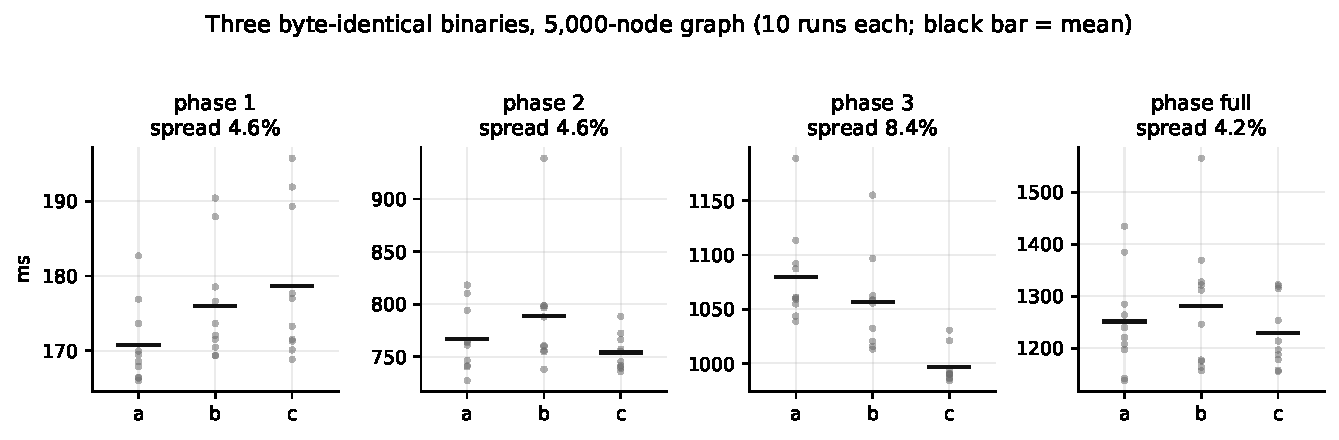
\includegraphics[width=\textwidth]{figures/fig1_null_test.pdf}
\caption{Three byte-identical binaries, 5{,}000-node graph, 10 runs each. All
spread here is ordering, thermal, and per-run variance --- the source code is
the same program. The worst case, $8.4\%$ in phase 3, is the floor we hold
claimed speedups against.}
\label{fig:null}
\end{figure}

The largest disagreement between identical programs is $8.4\%$, and we use that
conservative figure rather than the $4.2\%$ end-to-end value as the threshold
for a meaningful result. Note that this is substantially larger than the
within-command standard deviation, which is around $1.5\%$ end-to-end; reporting
only the latter would overstate confidence.

\subsection{Where baseline time goes}

Table~\ref{tab:composition} and Figure~\ref{fig:composition} give the baseline
phase composition at both graph sizes. Parsing, measured separately with
GraphViz's \texttt{gc} tool, accounts for $11.9 \pm 0.4$\,ms at 5{,}000 nodes
--- about $1\%$ of runtime --- and is included in the ranking figure below.

\begin{table}[htbp]
\centering
\caption{Baseline runtime composition, by differencing adjacent cumulative
phases. Crossing minimization dominates at 5{,}000 nodes; coordinate assignment
overtakes it at 10{,}000.}
\label{tab:composition}
\begin{tabular}{lrrrr}
\toprule
& \multicolumn{2}{c}{\textbf{5{,}000 nodes}} & \multicolumn{2}{c}{\textbf{10{,}000 nodes}} \\
\cmidrule(lr){2-3}\cmidrule(lr){4-5}
\textbf{Stage} & \textbf{ms} & \textbf{share} & \textbf{ms} & \textbf{share} \\
\midrule
Ranking                & 198.8  & 17.8\% & 214.7  & 6.2\%  \\
Crossing minimization  & 549.9  & 49.3\% & 1312.5 & 37.7\% \\
Coordinate assignment  & 252.5  & 22.6\% & 1697.6 & 48.7\% \\
Spline routing         & 114.6  & 10.3\% & 261.2  & 7.5\%  \\
\midrule
Total                  & 1115.7 & 100\%  & 3486.0 & 100\%  \\
\bottomrule
\end{tabular}
\end{table}

\begin{figure}[htbp]
\centering
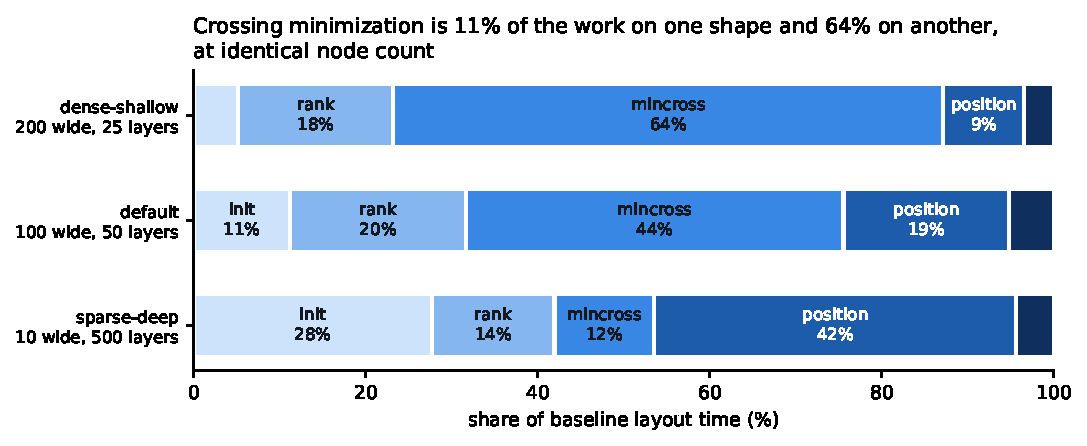
\includegraphics[width=\textwidth]{figures/fig2_phase_composition.pdf}
\caption{Baseline runtime composition at both graph sizes.}
\label{fig:composition}
\end{figure}

The shift is the important part. Crossing minimization falls from $49.3\%$ to
$37.7\%$ of runtime as the graph doubles, while coordinate assignment rises from
$22.6\%$ to $48.7\%$ and becomes dominant. Both are solved with network simplex
in the coordinate case; the crossing phase is an iterative heuristic. This
reweighting drives the divergence reported in Section~\ref{sec:scaling}.

\subsection{End-to-end results}

Table~\ref{tab:phases} gives cumulative phase timings for all three binaries at
both sizes, and Figure~\ref{fig:endtoend} plots the end-to-end result with every
individual run shown.

\begin{table}[htbp]
\centering
\caption{Cumulative phase timings, mean $\pm$ standard deviation over 10 runs.
Phases are cumulative: each row includes everything above it. All three
binaries were measured in one \texttt{hyperfine} invocation per row.}
\label{tab:phases}
\begin{tabular}{llrrr}
\toprule
\textbf{Graph} & \textbf{Phase} & \textbf{Baseline} & \textbf{Claude} & \textbf{Codex} \\
\midrule
\multirow{4}{*}{5{,}000}
 & 1 (ranking)              & $198.8 \pm 18.4$  & $184.5 \pm 14.9$  & $173.9 \pm 8.8$  \\
 & 2 (+ crossing min.)      & $748.7 \pm 27.6$  & $476.9 \pm 23.2$  & $572.9 \pm 20.1$ \\
 & 3 (+ coordinates)        & $1001.2 \pm 27.0$ & $640.2 \pm 23.7$  & $840.2 \pm 28.2$ \\
 & full (+ splines)         & $1115.7 \pm 16.2$ & $\mathbf{758.9 \pm 19.9}$ & $\mathbf{960.9 \pm 27.1}$ \\
\midrule
\multirow{4}{*}{10{,}000}
 & 1 (ranking)              & $214.7 \pm 1.4$    & $214.4 \pm 2.4$   & $221.1 \pm 11.4$  \\
 & 2 (+ crossing min.)      & $1527.2 \pm 20.0$  & $978.3 \pm 19.2$  & $1245.9 \pm 42.5$ \\
 & 3 (+ coordinates)        & $3224.8 \pm 214.1$ & $2109.1 \pm 74.7$ & $2720.6 \pm 151.9$ \\
 & full (+ splines)         & $3486.0 \pm 263.4$ & $\mathbf{2226.6 \pm 26.2}$ & $\mathbf{3028.9 \pm 292.3}$ \\
\bottomrule
\end{tabular}
\end{table}

\begin{figure}[htbp]
\centering
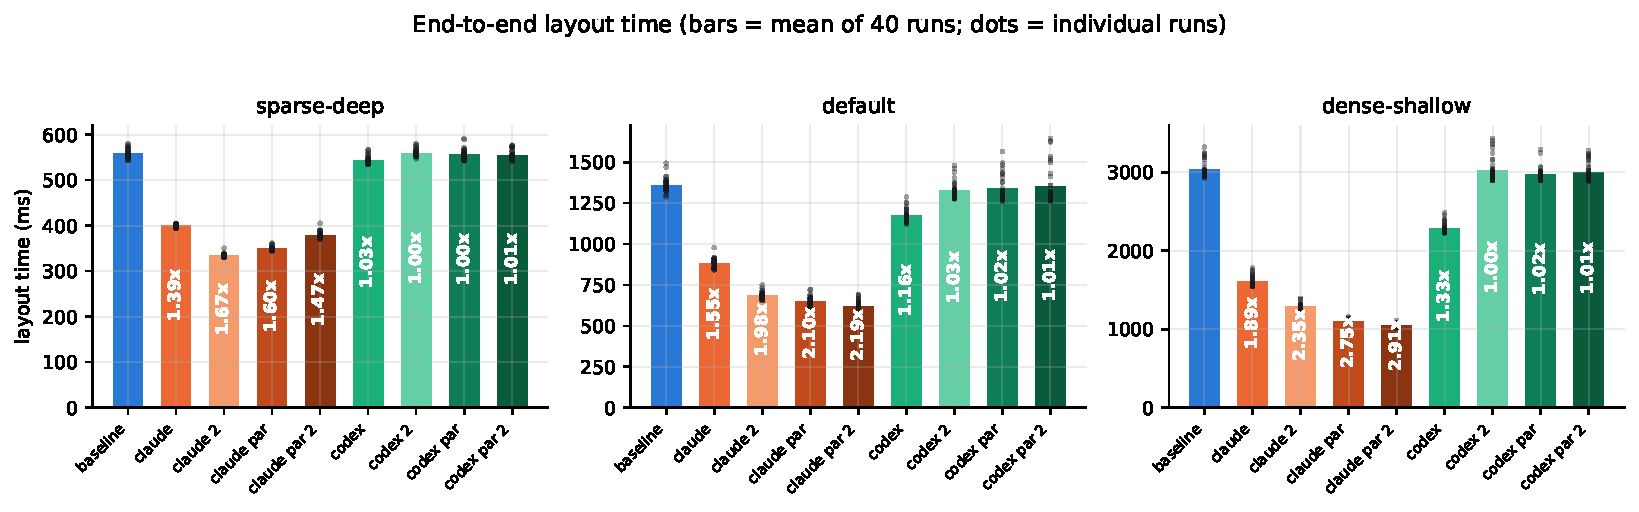
\includegraphics[width=\textwidth]{figures/fig3_end_to_end.pdf}
\caption{End-to-end layout time. Bars are means of 10 runs; dots are the
individual runs.}
\label{fig:endtoend}
\end{figure}

At 5{,}000 nodes Claude reaches $1.47\times$ and Codex $1.16\times$ end-to-end.
Both exceed the $8.4\%$ floor, Claude by a wide margin. Codex's $16\%$
improvement is roughly twice the floor: real, but a margin worth stating
explicitly rather than reporting as a bare ratio.

\subsection{Per-stage attribution}

\begin{table}[htbp]
\centering
\caption{Per-stage speedup over baseline, derived by differencing adjacent
phases. Differencing compounds the error of both terms; these are weaker
evidence than Table~\ref{tab:phases}.}
\label{tab:stages}
\begin{tabular}{lrrrr}
\toprule
& \multicolumn{2}{c}{\textbf{5{,}000 nodes}} & \multicolumn{2}{c}{\textbf{10{,}000 nodes}} \\
\cmidrule(lr){2-3}\cmidrule(lr){4-5}
\textbf{Stage} & \textbf{Claude} & \textbf{Codex} & \textbf{Claude} & \textbf{Codex} \\
\midrule
Ranking               & 1.08$\times$ & 1.14$\times$ & 1.00$\times$ & 0.97$\times$ \\
Crossing minimization & 1.88$\times$ & 1.38$\times$ & 1.72$\times$ & 1.28$\times$ \\
Coordinate assignment & 1.55$\times$ & 0.94$\times$ & 1.50$\times$ & 1.15$\times$ \\
Spline routing        & 0.97$\times$ & 0.95$\times$ & ---          & ---          \\
\bottomrule
\end{tabular}
\end{table}

Figure~\ref{fig:perrun} shows every run at 5{,}000 nodes. The ranking phase is
the cautionary case: the three binaries lie within about 25\,ms of one another
on a measurement whose per-binary standard deviation is 9--18\,ms, and their
distributions overlap almost completely. We report ranking as no difference.
Neither agent modified the ranking path in a way that would be expected to
matter here, since the generated graphs pin ranks explicitly and leave little
ranking work to do.

Spline routing at 10{,}000 nodes is omitted from Table~\ref{tab:stages}. It is
derived by subtracting two quantities whose standard deviations are 214\,ms and
263\,ms, and the resulting figure is not meaningful.

\begin{figure}[htbp]
\centering
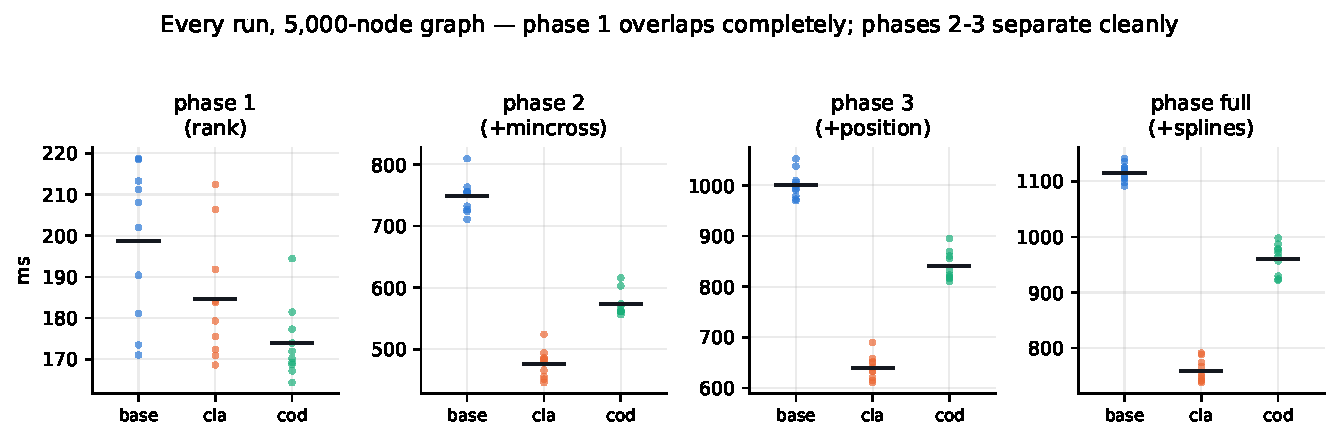
\includegraphics[width=\textwidth]{figures/fig4_per_run_distributions.pdf}
\caption{All 10 runs per binary per phase, 5{,}000-node graph. The ranking
phase overlaps completely across all three binaries; phases 2 and 3 separate
cleanly.}
\label{fig:perrun}
\end{figure}

\subsection{Scaling}
\label{sec:scaling}

\begin{figure}[htbp]
\centering
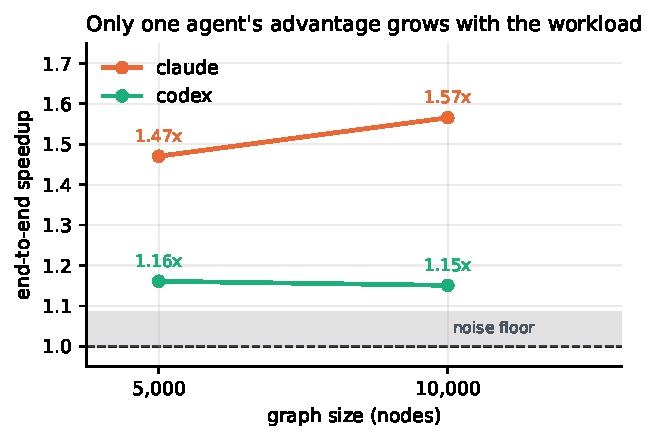
\includegraphics[width=0.62\textwidth]{figures/fig5_scaling.pdf}
\caption{End-to-end speedup against graph size, with the noise floor shaded.
Two points are suggestive, not a fitted trend.}
\label{fig:scaling}
\end{figure}

Doubling the graph separates the two agents (Figure~\ref{fig:scaling}). Claude
improves from $1.47\times$ to $1.57\times$; Codex is flat, $1.16\times$ to
$1.15\times$. Table~\ref{tab:stages} shows the mechanism: at 10{,}000 nodes
coordinate assignment is $48.7\%$ of runtime, and Claude achieves $1.50\times$
on it against Codex's $1.15\times$.

\subsection{What the agents changed}

Both agents modified crossing minimization, and both arrived independently at
the same core idea: the two symmetric crossing-count computations for an
adjacent node pair can be fused into a single pass, since any pair of incident
edges contributes to at most one of the two counts.

\textbf{Codex} made two code commits touching only
\texttt{lib/dotgen/mincross.c} (+122/$-$17 lines). Beyond the fused counts, it
replaced a linear prefix scan in the crossing-count routine with a Fenwick tree,
reducing that inner loop from $O(n)$ to $O(\log n)$.

\textbf{Claude} made eight code commits touching
\texttt{lib/dotgen/mincross.c} and \texttt{lib/common/ns.c} (+978/$-$169 lines).
It found the same fused-count transformation, then restructured the network
simplex implementation: the depth-first traversal keeps its current frame in
local variables backed by a reusable stack, and the scattered per-node fields
reached through accessor macros were replaced by a dense 32-byte-per-node state
array with cached neighbour pointers. This is a memory-locality change, and it
is what produces the coordinate-assignment improvement in
Table~\ref{tab:stages}.

\subsection{Correctness}

Both agents' binaries produce \texttt{dot -Tdot} output byte-identical to the
baseline on the evaluation graphs (SHA-1 \texttt{3560c5d0\ldots} at 5{,}000
nodes). We read both diffs against the prompt's list of disallowed shortcuts and
found no reduced iteration counts, early exits, input special-casing, or
modified tests. Neither diff contains any OpenMP directive, thread creation, or
other concurrency construct.
